%TEMPLATE INFORMES LATEX

%IMPORTACIÓN DE LIBRERÍAS
%----------------------------------

\documentclass[11pt,a4paper]{article}
\usepackage[utf8]{inputenc}
\usepackage[spanish]{babel}
\usepackage{amsmath}
\usepackage{natbib}
\usepackage{amsfonts}
\usepackage{amssymb}
\usepackage{graphicx}
\usepackage{listings}
\usepackage{longtable}
\usepackage{subfig}
\usepackage{subfigure}
\usepackage{makeidx}
\usepackage{multirow}
\usepackage{url}
\usepackage{biblatex} %Imports biblatex package
\usepackage{color} %red, green, blue, yellow, cyan, magenta, black, white
\definecolor{mygreen}{RGB}{28,172,0} % color values Red, Green, Blue
\definecolor{mylilas}{RGB}{170,55,241}
\definecolor{gray}{RGB}{220,220,220}
\lstset{language=Matlab,%
    %basicstyle=\color{red},
    breaklines=true,%
    morekeywords={matlab2tikz},
    keywordstyle=\color{blue},%
    morekeywords=[2]{1}, keywordstyle=[2]{\color{black}},
    identifierstyle=\color{black},%
    stringstyle=\color{mylilas},
    commentstyle=\color{mygreen},%
    showstringspaces=false,%without this there will be a symbol in the places where there is a space
    numbers=left,%
    numberstyle={\tiny \color{black}},% size of the numbers
    numbersep=9pt, % this defines how far the numbers are from the text
    emph=[1]{for,end,break},emphstyle=[1]\color{red}, %some words to emphasise
    %emph=[2]{word1,word2}, emphstyle=[2]{style},    
}
\usepackage[left=2cm,right=2cm,top=2cm,bottom=2cm]{geometry}
\usepackage{enumerate}
\usepackage{float}
\usepackage{pdfpages}
%Estilo de página
\usepackage{fancyhdr}
\pagestyle{fancy}

    \usepackage{wrapfig}
    \usepackage{color}
    \definecolor{rojo}{RGB}{255,26,34}
    \definecolor{gris}{RGB}{104,108,113}
    \newcommand{\HRule}{\rule{\linewidth}{.4mm}}
    %figuras .eps
    \usepackage{epstopdf}
    %\epstopdfsetup{update}
    \usepackage{hyperref}
    %agregar .m
    %\usepackage[numbered,framed]{mcode}
    %\usepackage{listings}
    \addto\captionsenglish{\renewcommand{\figurename}{Figura}}
    \usepackage[table]{xcolor}
    \usepackage{indentfirst}
\usepackage{etoolbox}
\usepackage[utf8]{inputenc}
\usepackage{array}
\graphicspath{ {figures/} }

%IMPORTAR BIBLIOGRAFÍA
%----------------------------------
\addbibresource{bibliografia.bib} 
\bibliographystyle{ieee}
%INICIO DEL DOCUMENTO
%----------------------------------
\begin{document}
\renewcommand{\tablename}{Tabla}


%TÍTULO Y ENCABEZADOS ---------------------------------
\begin{titlepage}

%ENCABEZADO DE PORTADA
%---------------------------------
{
\begin{wrapfigure}{l}{.8cm}
\vspace{-.7cm}

\includegraphics[width=4.7cm]{img/fcfm}
\end{wrapfigure}
\textsc{\color{red}\hspace{3cm}Universidad de Chile}\\
\textsc{\color{gray}\hspace{3.6cm}Facultad de Ciencias Físicas y Matemáticas}\\
\textsc{\color{gray}\hspace{3.6 cm}Departamento de Ingeniería Eléctrica}\\
\textsc{\color{gray}\hspace{3.6cm}\small EL7030 - Antenas}\\
}
%ENCABEZADO DE OTRAS PÁGINAS
%--------------------------------
\fancyhead[l]{\small EL7030 - Antenas - 2024/1}
\fancyhead[r]{
\includegraphics[scale=0.1]{img/fcfm}}
    
% TITULO 
--------------------------------
        \begin{center}
        ~\\[3.5cm]
        \HRule~ \\[0.4cm]
        { \Huge \textup \bfseries  Tarea 3: Diseño de antena Moxon adaptada para la recepción de señales NOAA}\\[0.4cm]
        { \Large \textup{EL7030 - Antenas}}\\[0.2cm]
        \HRule ~\\[2cm]
        \end{center}
        \begin{minipage}{.5\textwidth}
       
        \end{minipage}
    
%INTEGRANTES
    ~\\[2cm]
    ~ ~ ~
    \begin{minipage}{.8\textwidth}
    \begin{flushright}
    \begin{tabular}{l}
        
        \emph{Profesor:} \\
            {\small Ricardo Finger C.} \\
        \\[0.29cm]

        \emph{Profesor auxiliar:} \\
            {\small Juan Torrejon H.} \\
            {\small Vicente Aitken A.} \\
        \\[0.29cm]
        
        %\emph{Ayudantes:} \\
        %    {\small Camila Maire} \\
        %    {\small Ricardo García R.} \\
        %    {\small Valeria C. Zúñiga} \\
        %\\[0.29cm]

        \emph{Estudiante:} \\
            {\small Maximiliano Morales
            H.} \\
            {\small Erik Sáez Aravena}\\
        \\[0.29cm] 
        
        \emph{Fecha de entrega:} \\
            {\small \today}
        \\[0.29cm]  

    \end{tabular}
    \end{flushright}
    \end{minipage}
    
\end{titlepage}

\newpage

%TABLA DE CONTENIDOS-------------------------
\renewcommand{\contentsname}{Índice.}
\tableofcontents{}
\newpage

%LISTA DE FIGURAS Y TABLAS-------------------------
\renewcommand{\listfigurename}{Lista de figuras.}
\renewcommand{\listtablename}{Lista de tablas.}
\listoffigures
\listoftables
\pagenumbering{arabic}

\newpage
\section{Marco teórico}
\subsection{Protocolo NOAA-APT}
El protocolo NOAA (National Oceanic and Atmospheric Administration) se refiere a los satélites meteorológicos operados por esta agencia estadounidense que recopilan y transmiten datos atmosféricos, climáticos y medioambientales. Estos satélites son parte de la serie de satélites polar y geosíncronos que capturan imágenes y datos a nivel global. Los satélites NOAA emiten en diversas frecuencias, principalmente en bandas VHF y UHF, para proporcionar imágenes en tiempo real a estaciones de recepción terrestre.\\
En la tabla \ref{tab:noaa_frequencies} se adjunta la serie de satélites NOAA que fueron/han utilizado a lo largo de los años conjunto con sus frecuencias de operación y tipo de transmisión \cite{noaaProyecto}.

\begin{table}[h!]
    \centering
    \begin{tabular}{|c|c|c|c|}
        \hline
        \parbox[c][1cm][c]{3cm}{\centering Satélite} & \parbox[c][1cm][c]{4cm}{\centering Frecuencia de transmisión (MHz)} & \parbox[c][1cm][c]{2cm}{\centering Banda} & \parbox[c][1cm][c]{4cm}{\centering Tipo de transmisión} \\
        \hline
        NOAA-15 & 137.620 & VHF & HRPT / HRPT \\
        \hline
        NOAA-16 & 137.620 & VHF & APT / HRPT \\
        \hline
        NOAA-17 & 137.500 & VHF & APT \\
        \hline
        NOAA-18 & 137.912 & VHF & APT \\
        \hline
        NOAA-19 & 137.100 & VHF & APT \\
        \hline
    \end{tabular}
    \caption{Frecuencias de transmisión de los satélites NOAA-15, NOAA-16, NOAA-17, NOAA-18 y NOAA-19.}
    \label{tab:noaa_frequencies}
\end{table}

Cabe mencionar que debido a desperfectos técnicos, solamente NOAA-15, 18 Y 19 se encuentran operativos según \cite{noaaSatellites}.


\subsection{Formato APT}
El APT (Automatic Picture Transmission) corresponde al formato de transmisión de los satélites NOAA el cual corresponde a una modulación en amplitud de una subportadora de 2400 Hz con los 8 bits más significativos de la señal digital de 10 bits
Datos AVHRR. Los datos AVHRR (Advanced Very High Resolution Radiometer) son un tipo de información captada por un sensor multiespectral instalado en los satélites. De los 6 canales espectrales posibles que captura el AVHRR, solo se seleccionan 2 para transmitir en el APT. Estos dos canales se envían de forma alternada: uno en el canal A y otro en el canal B. Las estaciones en tierra deciden qué canales transmitir, pero el usuario no puede seleccionar qué canales recibir. Dado que el sistema APT no transmite todos los datos (solo 1/3 de las líneas de escaneo por minuto), la resolución de las imágenes es más baja que los datos originales de AVHRR. Sin embargo, sigue siendo suficiente para proporcionar imágenes en tiempo real con una tasa de 120 líneas de video por minuto \cite{noaaReceiveStations}.\\

En la figura \ref{fig:apt} se presenta el formato de transmisión de video para APT.

\begin{figure}[h!]
    \centering
    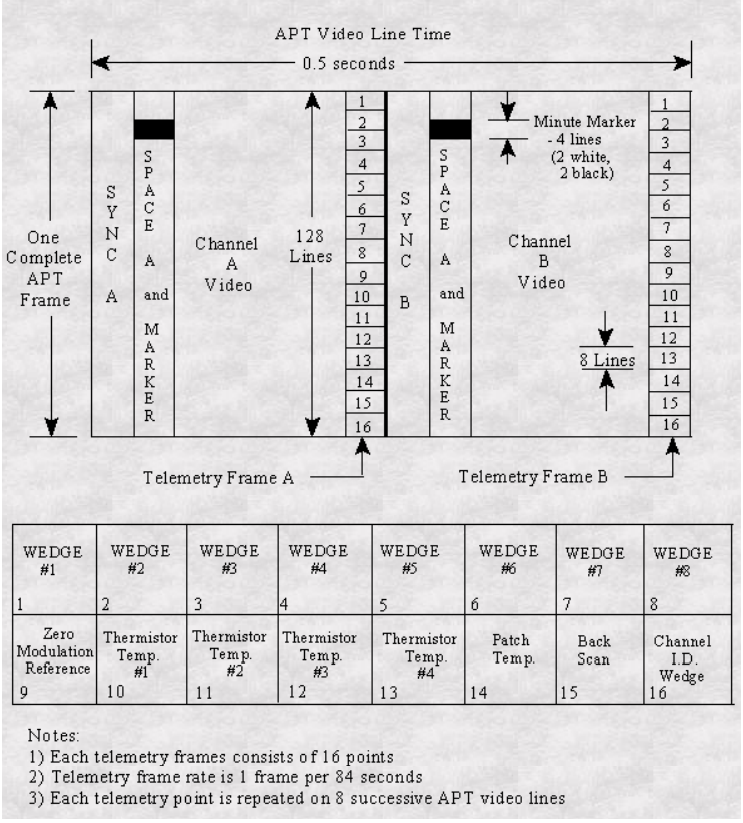
\includegraphics[width=0.7\linewidth]{img/apt.png}
    \caption{Formato de un frame APT.}
    \label{fig:apt}
\end{figure}

El resultado es la recepción de un frame como se presenta a continuación en la figura \ref{fig:imagen_frame}.

\begin{figure}[h!]
    \centering
    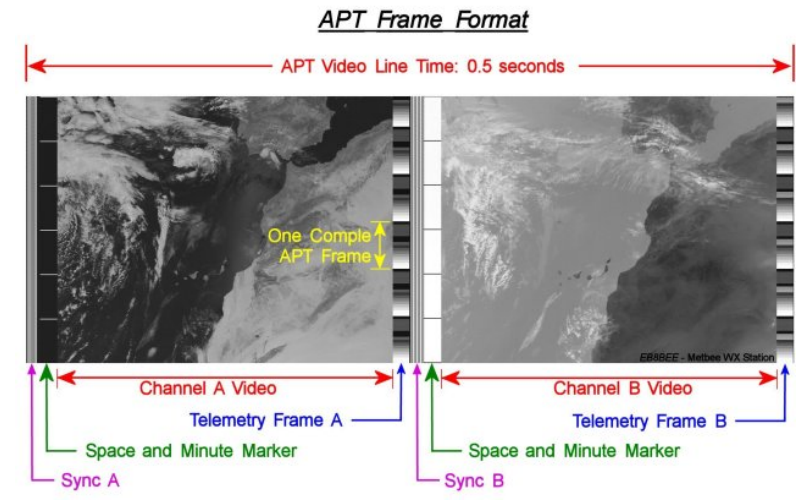
\includegraphics[width=0.7\linewidth]{img/result.png}
    \caption{Ejemplo de frame recibido según un formato APT}
    \label{fig:imagen_frame}
\end{figure}

\subsection{Antenas adaptadas a NOAA-APT}
Para la elección de la antena que sería utilizada en esta experiencia, se investigó de forma exhaustiva en la literatura posibles antenas candidatas tomando en cuenta como directriz obtener la imagen de mayor calidad. Para ello, basado en el trabajo realizado en \cite{PazPenagos2024} se opta por escoger la antena Moxon por su facil diseño de contrucción y el buen rendimiento en cuanto a calidad de imagen recibida respecto a otras antenas. En efecto, en la figura \ref{fig:antenas_paper} se presenta las imágenes obtenidas para las distintas antenas que se utilizaron en el paper.

\begin{figure}[h!]
    \centering
    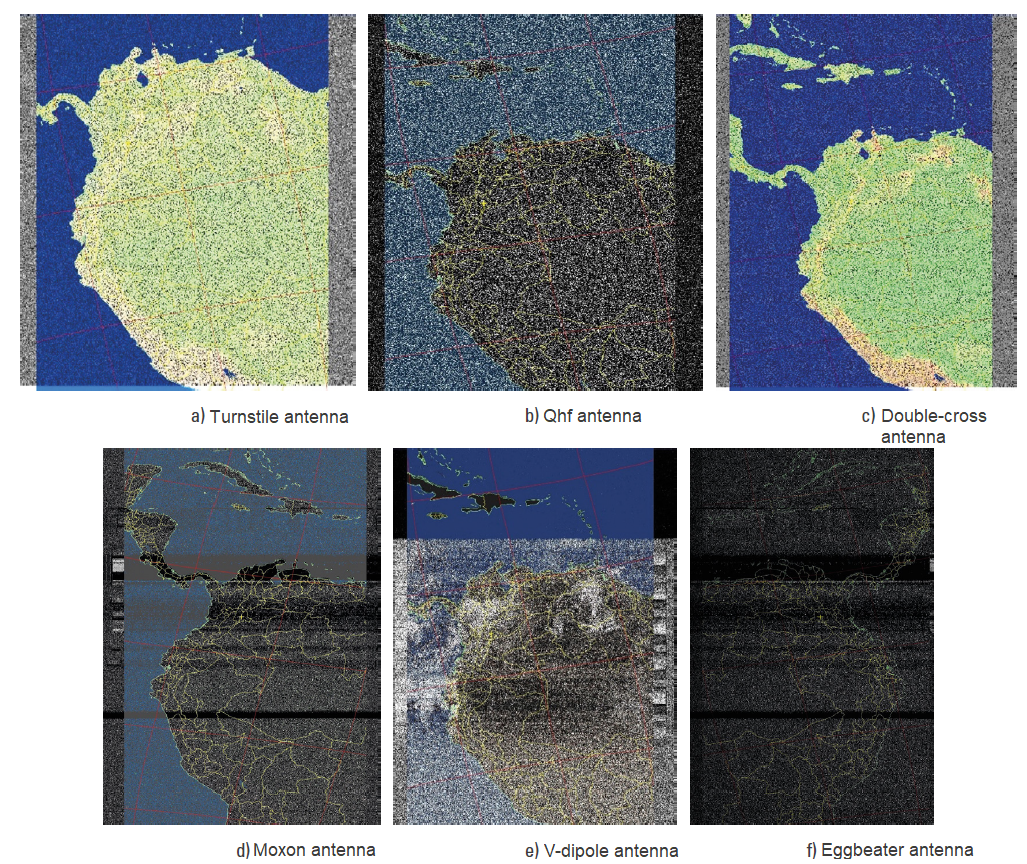
\includegraphics[width=0.7\linewidth]{img/antenas.png}
    \caption{Imágenes obtenidas por las distintas antenas que fueron utilizadas en el paper de referencia.}
    \label{fig:antenas_paper}
\end{figure}


En la tabla \ref{tab:resolucion_senal} se presenta los resultados cuantitativos en cuanto a resolución y potencia recibida. La antena Moxon destaca por su buena resolución $1,94$ megapixéles mientras que la QFH lo hace por su buena recepción de peak de potencia igual a $1.9$ W.

\begin{table}[h]
    \centering
    \begin{tabular}{|c|c|c|c|c|}
        \hline
        \parbox[c][2cm][c]{2cm}{\centering Imagen} & \parbox[c][2cm][c]{2.5cm}{\centering Resolución (megapíxeles)} & \parbox[c][2cm][c]{2.5cm}{\centering Píxeles en el eje vertical} & \parbox[c][2cm][c]{2.5cm}{\centering Píxeles en el eje horizontal} & \parbox[c][2cm][c]{3cm}{\centering Potencia peak de la señal recuperada (mW)} \\
        \hline
        1a & 1,41544 & 1361 & 1040 & 863,23 \\
        \hline
        1b & 1,08056 & 1039 & 1040 & 1920,3 \\
        \hline
        1c & 1,4612  & 1405 & 1040 & 3,33 \\
        \hline
        1d & 1,93648 & 1862 & 1040 & 2,47 \\
        \hline
        1e & 1,43832 & 1383 & 1040 & 1264 \\
        \hline
        1f & 1,515544 & 1556 & 974 & 141,63 \\
        \hline
    \end{tabular}
    \caption{Resolución de imágenes y potencia de pico de la señal recuperada.}
    \label{tab:resolucion_senal}
\end{table}


\newpage


\subsection{Antena Móxon}
En la figura \ref{fig:antena_moxon} se presenta el diagrama de una antena Moxon. 

\begin{figure}
    \centering
    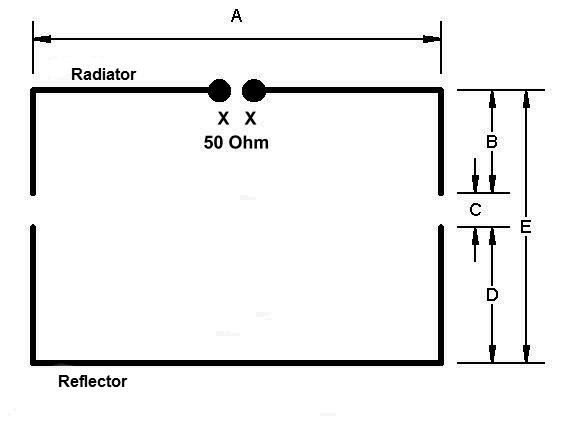
\includegraphics[width=0.55\linewidth]{img/moxon.png}
    \caption{Diagrama de antena Moxon.}
    \label{fig:antena_moxon}
\end{figure}

Por otra parte, las dimensiones de la antena moxon (figura \ref{fig:antena_moxon}) se calcula para una longitud de onda en particular $\lambda$ según la tabla \ref{tab:antena_dimensiones} (ver \cite{moxonAntenna} para más detalles). 

\begin{table}[h!]
    \centering
    \begin{tabular}{|c|c|}
        \hline
        \textbf{Dimensión de la antena} & \textbf{Ecuación} \\
        \hline
        Dimensión $a$ & $a \approx 0.375 \cdot \lambda$ \\
        \hline
        Dimensión $b$ & $b \approx 0.0575 \cdot \lambda$ \\
        \hline
        Dimensión $c$ & $c \approx 0.0675 \cdot \lambda$ \\
        \hline
        Elemento activo & $a + 2b \approx 0.49 \cdot \lambda$ \\
        \hline
        Reflector & $a + 2c \approx 0.51 \cdot \lambda$ \\
        \hline
        Ganancia esperada & $\approx 5 \text{ dBi}$ \\
        \hline
        Relación frente-a-espalda & $\approx 20 \text{ dB}$ \\
        \hline
    \end{tabular}
    \caption{Dimensiones y ecuaciones de la antena.}
    \label{tab:antena_dimensiones}
\end{table}


\subsection{Simulaciones HFSS}
Para el diseño y posterior simulación de la antena en el software HFSS, para lo cual se utilizaron las siguiente medidas de la figura \ref{fig:dimensiones_moxon} que fueron optimizadas mediante parametrización de la antena:

\begin{figure}[h]
    \centering
    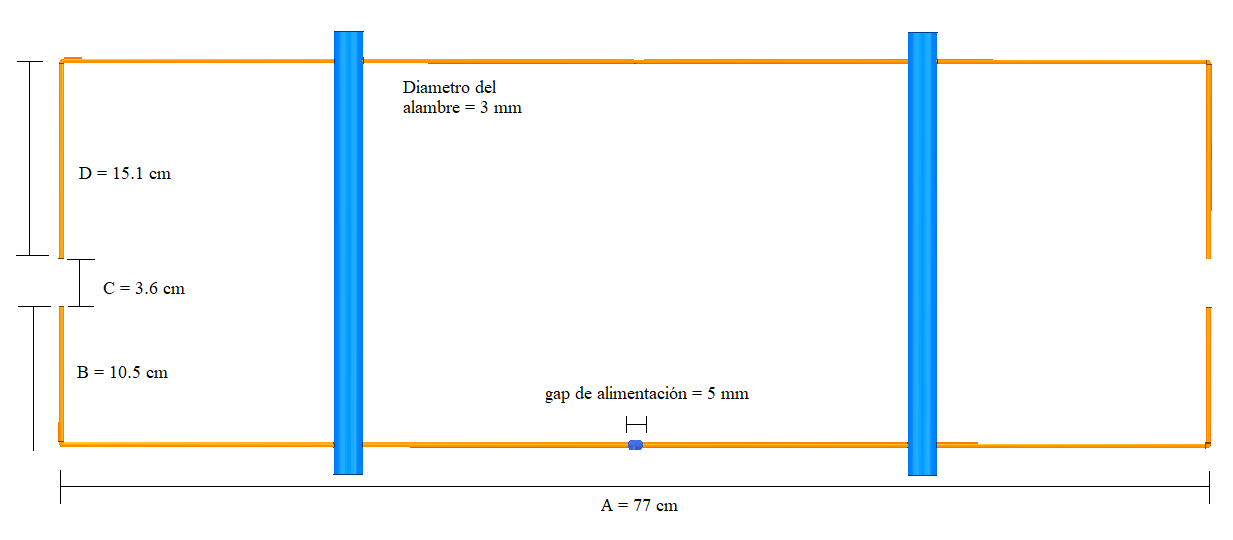
\includegraphics[width=0.85\linewidth]{img/dimensiones_moxon.png}
    \caption{Dimensiones antena Moxon simulada en HFFS con conexión LumpedPort. El material celeste corresponden a barras de PVC de 2 cm de diámetro y largo 33 cm. No se incluyen estos valores ya que a priori no toman mayor relevancia en el diseño de la antena más que proveer una estructura firme.}
    \label{fig:dimensiones_moxon}
\end{figure}

A continuación, el parámetro $S_{11}$ obtenido se presenta en la figura \ref{fig:hfss_s11}. Se observa que para la frecuencia necesaria para la sintonización de los satélites, $137.5$ Mhz se tienen aproximadamente -30[dB], lo cual es suficiente para el propósito del experimento.

\begin{figure}[H]
    \centering
    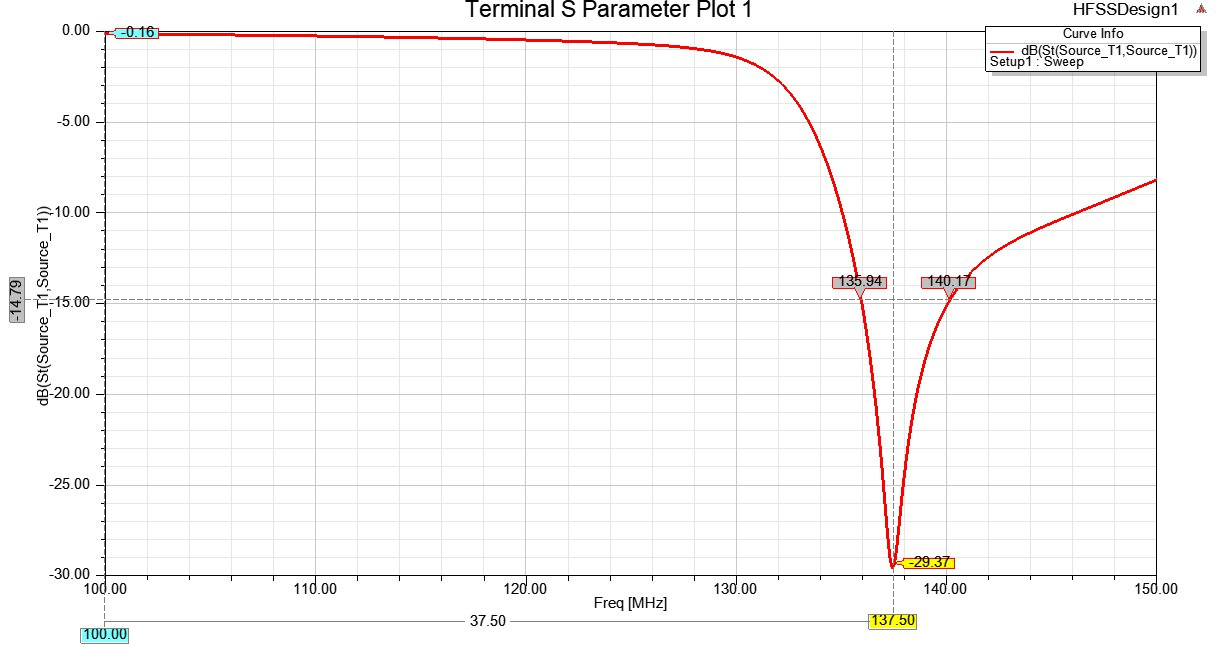
\includegraphics[width=0.7\linewidth]{img/s11.jpg}
        \caption{Parámetro $S_{11}$ de antena Moxon simulada en HFSS. La marca indica mínima ganancia (-30 dB) para la frecuencia 137.5 Mhz.}
    \label{fig:hfss_s11}
\end{figure}

Se presenta en la figura \ref{fig:gain3D} el patrón de radiación en 3D en decibeles. Se observa que presenta una ganancia de $6.2$[dB] lo cual es aceptable para el propósito de la experiencia.
\begin{figure}[H]
    \centering
    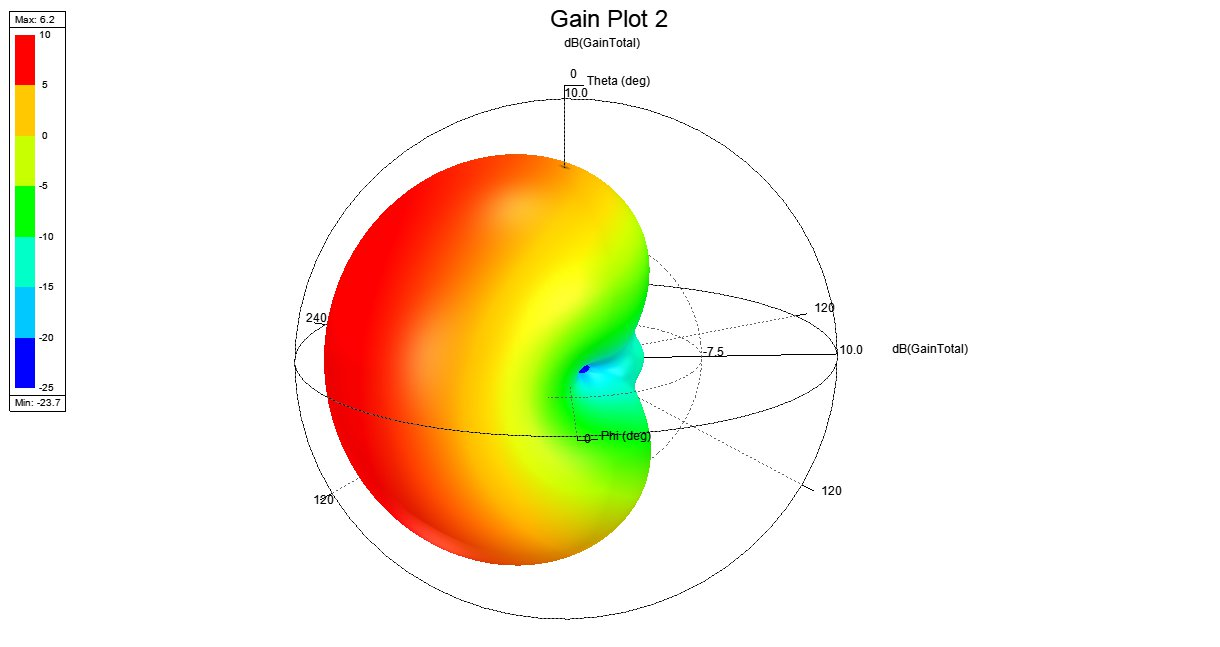
\includegraphics[width=0.7\linewidth]{img/Gain.jpg}
    \caption{Patrón de radiación en 3D indicando la ganancia en base a un mapa de colores donde se observa que presenta un maximo en 6.2[dB].}
    \label{fig:gain3D}
\end{figure}

Como se puede apreciar en la figura \ref{fig:gain3D}, la antena Moxon a diferencia de antenas típicas utilizadas para sintonizar frecuencias NOAA, es directiva por lo que será necesario conocer la dirección a la cual deberá colocarse para obtener la máxima ganancia al momento de recibir las señales APT. En la figura \ref{fig:patron_antena} se presenta la antena y el patrón de radiación en 3D.

\begin{figure}[h]
    \centering
    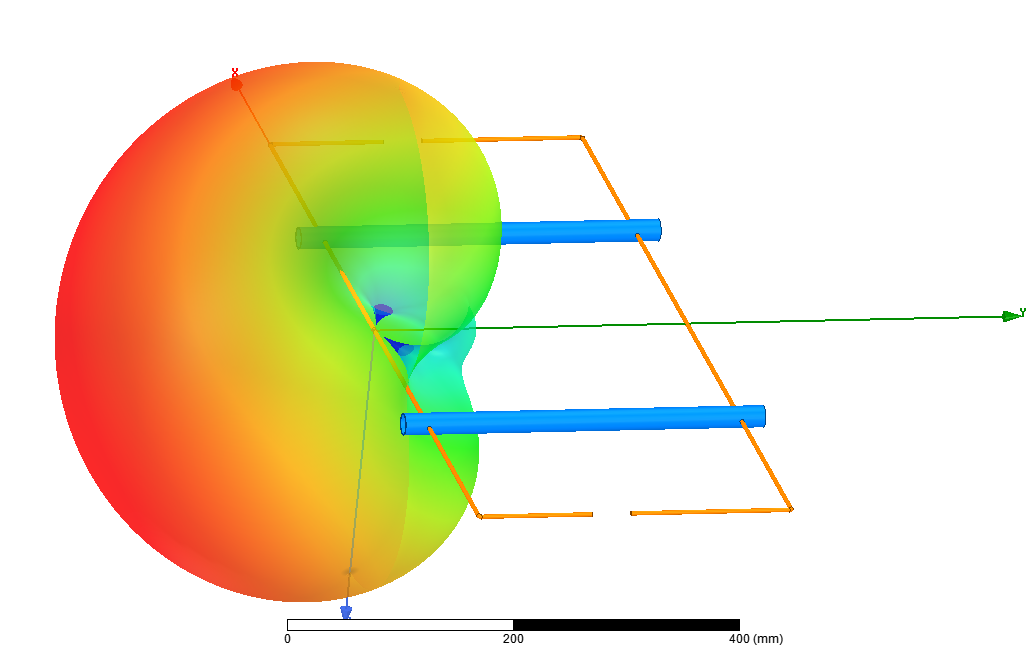
\includegraphics[width=0.5\linewidth]{img/patron_antena.png}
    \caption{Antena Moxon y su respectivo patrón de radiación superpuesto. Se observa que el patrón comienza desde el puerto de alimentación y se extiende hacia atrás de la antena en el eje Y.}
    \label{fig:patron_antena}
\end{figure}

En la figura \ref{fig:planosEH} se presenta el patrón de radiación en los planos E y H.

\begin{figure}
    \centering
    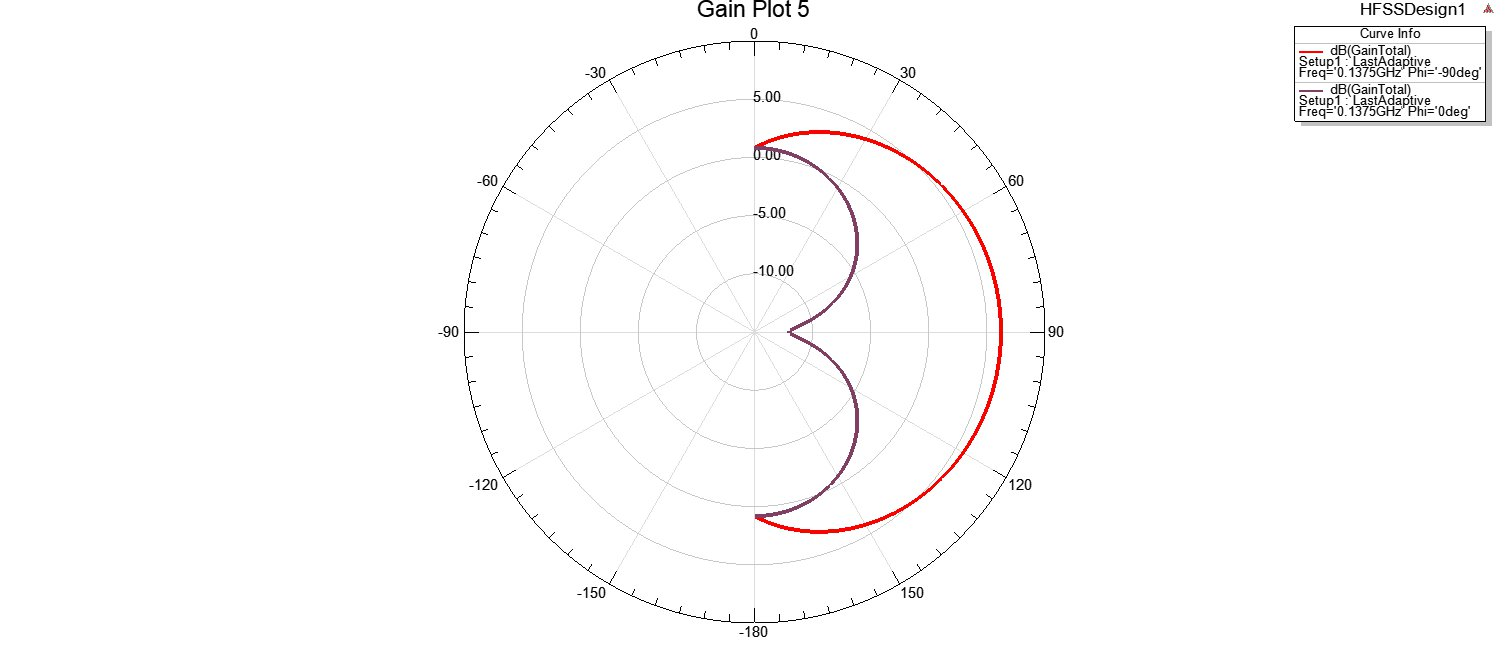
\includegraphics[width=0.5\linewidth]{img/planoEH.jpg}
    \caption{Planos E-Plane (café) y H-Plane (rojo) para la ganancia en un gráfico polar,}
    \label{fig:planosEH}
\end{figure}


\section{Resultados experimentales}
Siguiendo las dimensiones simuladas en la figura \ref{fig:dimensiones_moxon} se construye la antena Moxon. Se adjunta en la figura \ref{fig:antena_real} la antena ya fabricada.\\
\begin{figure}[h!]
    \centering
    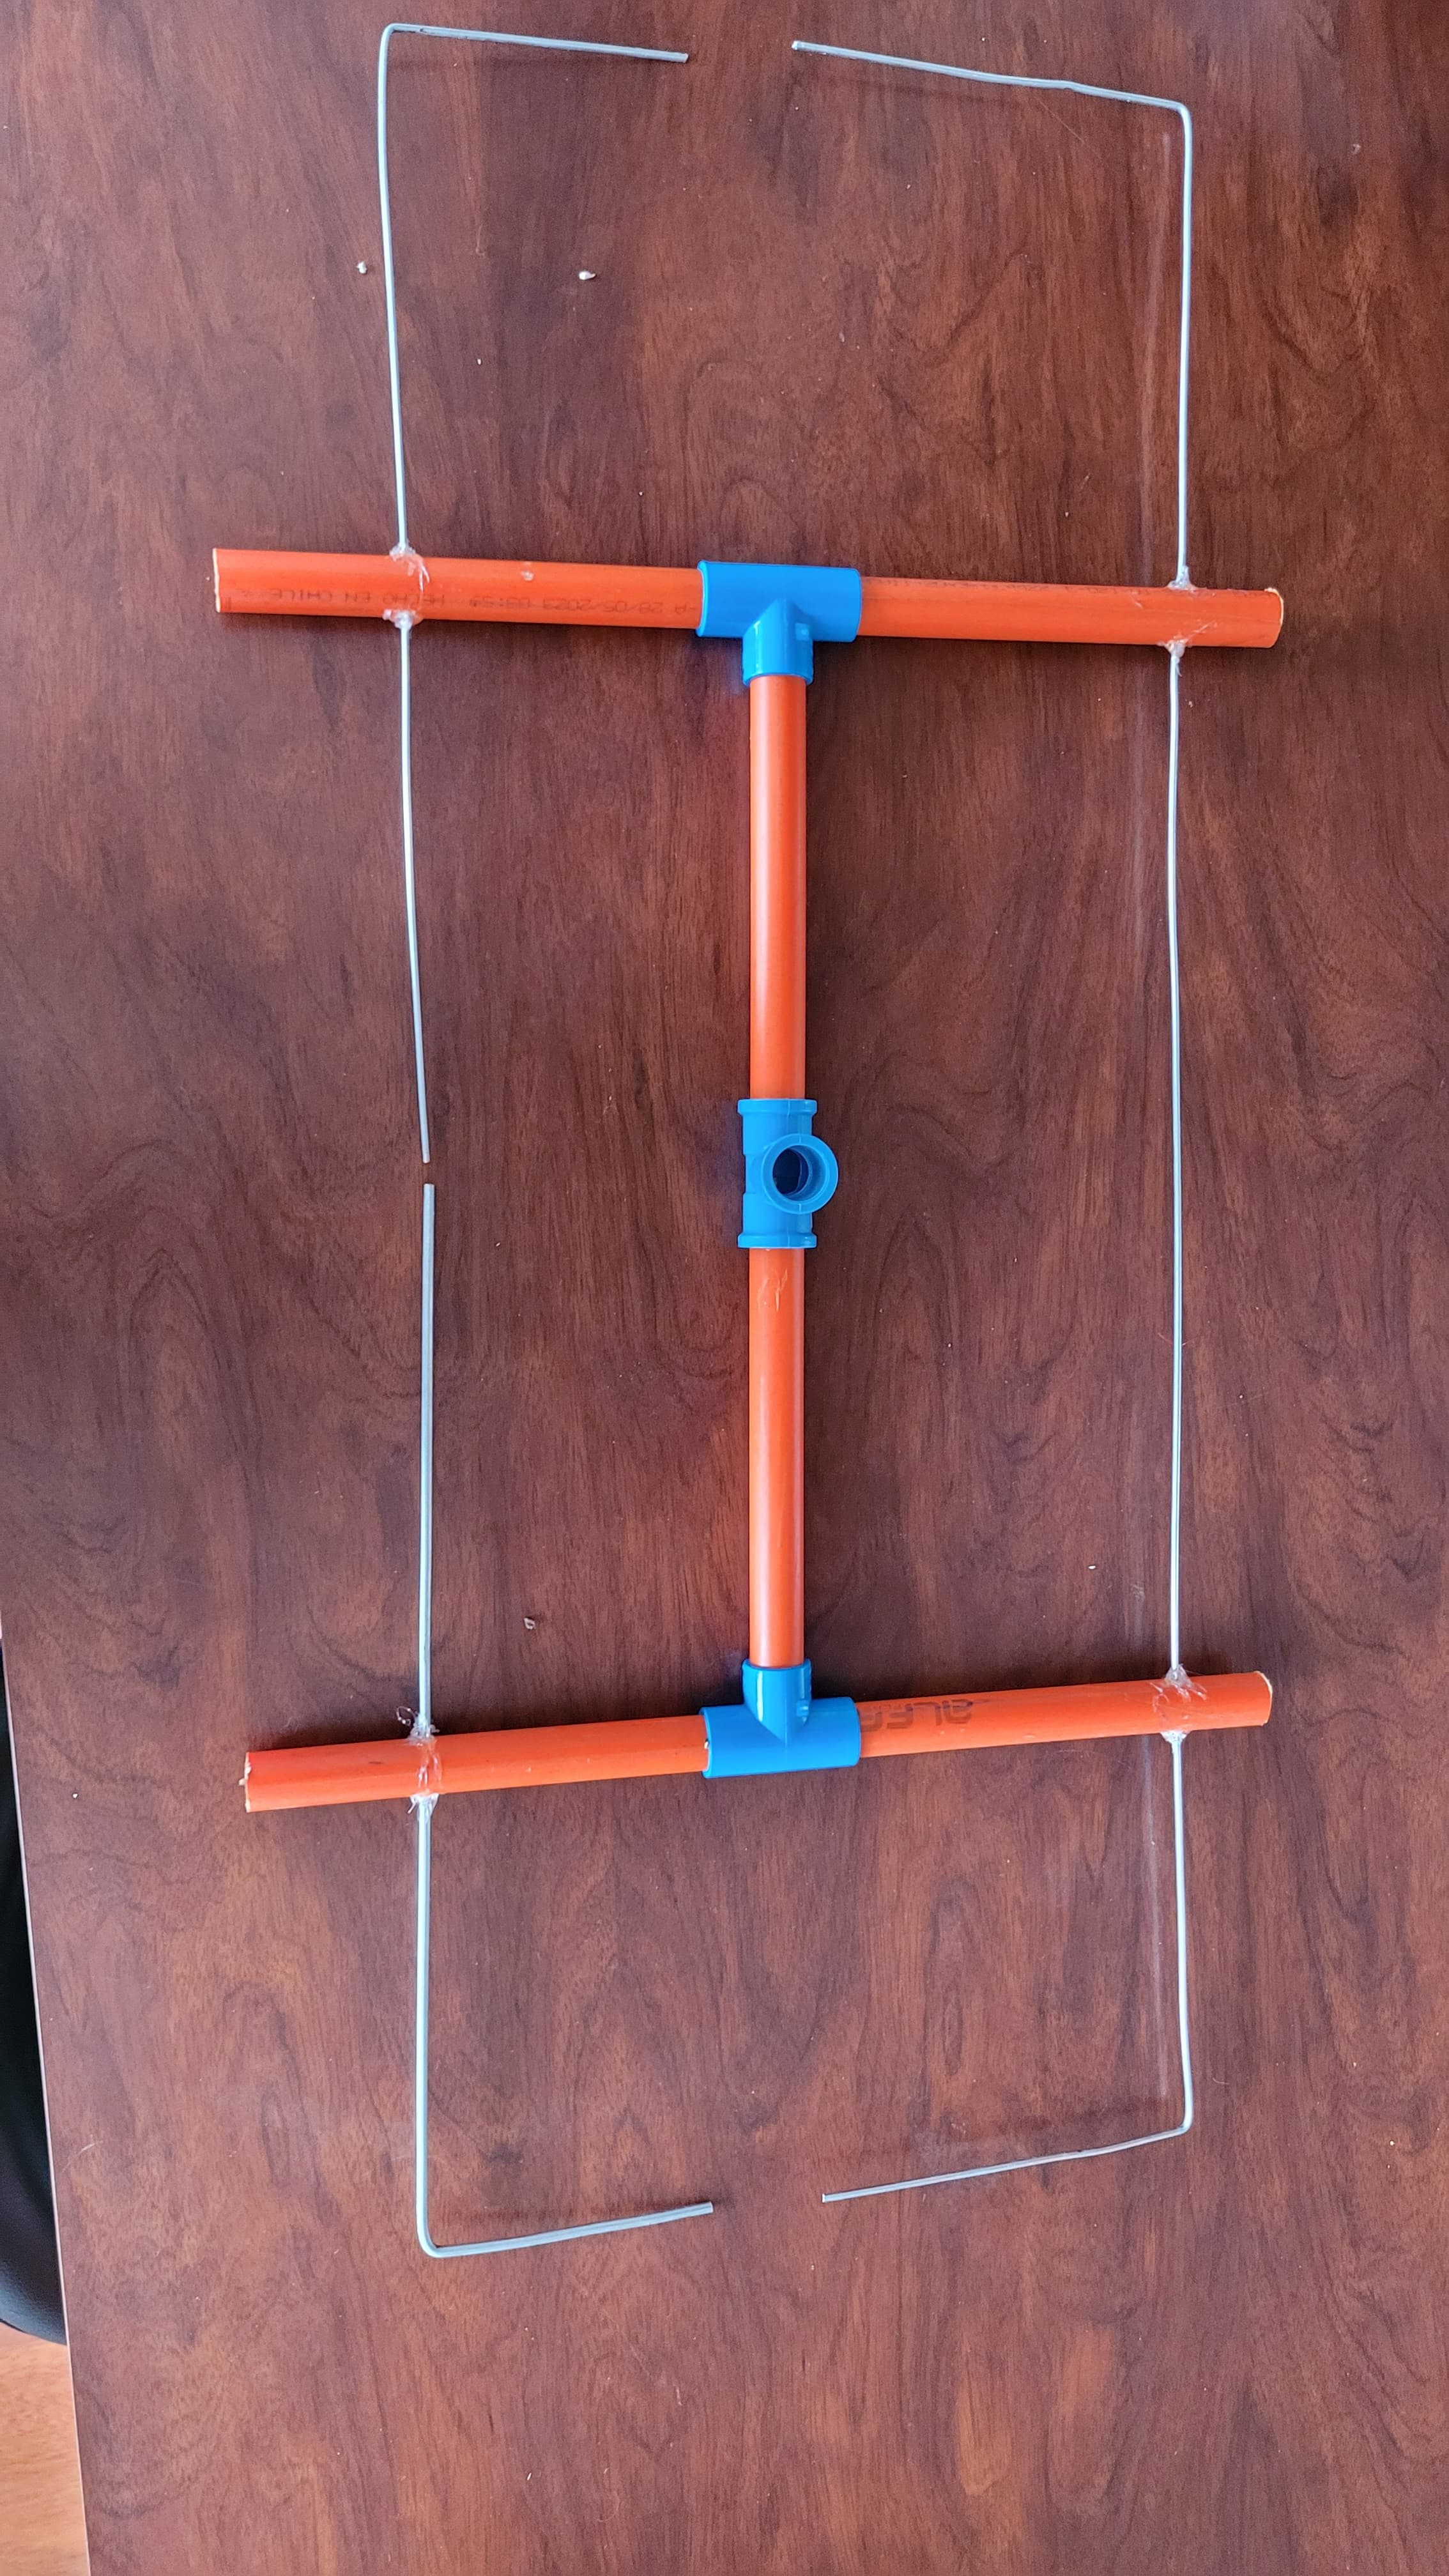
\includegraphics[width=0.4\linewidth, angle=90]{img/antena_real.jpeg}
    \caption{Antena Moxon fab}
    \label{fig:antena_real}
\end{figure}

\newpage
%\printbibliography
\end{document}
